\section{Identifying the Challenge}

\subsection*{Problem Definition}\begin{frame}\frametitle{Air Defence System Limitations}
    \begin{itemize}
        \item Air defense systems are vital for protection against air attacks.
        \item Complex systems require extensive research to perform well.
        \pause
        \item Limitations exist that cannot be addressed by merely improving internal algorithms.
        \begin{figure}
            \centering
            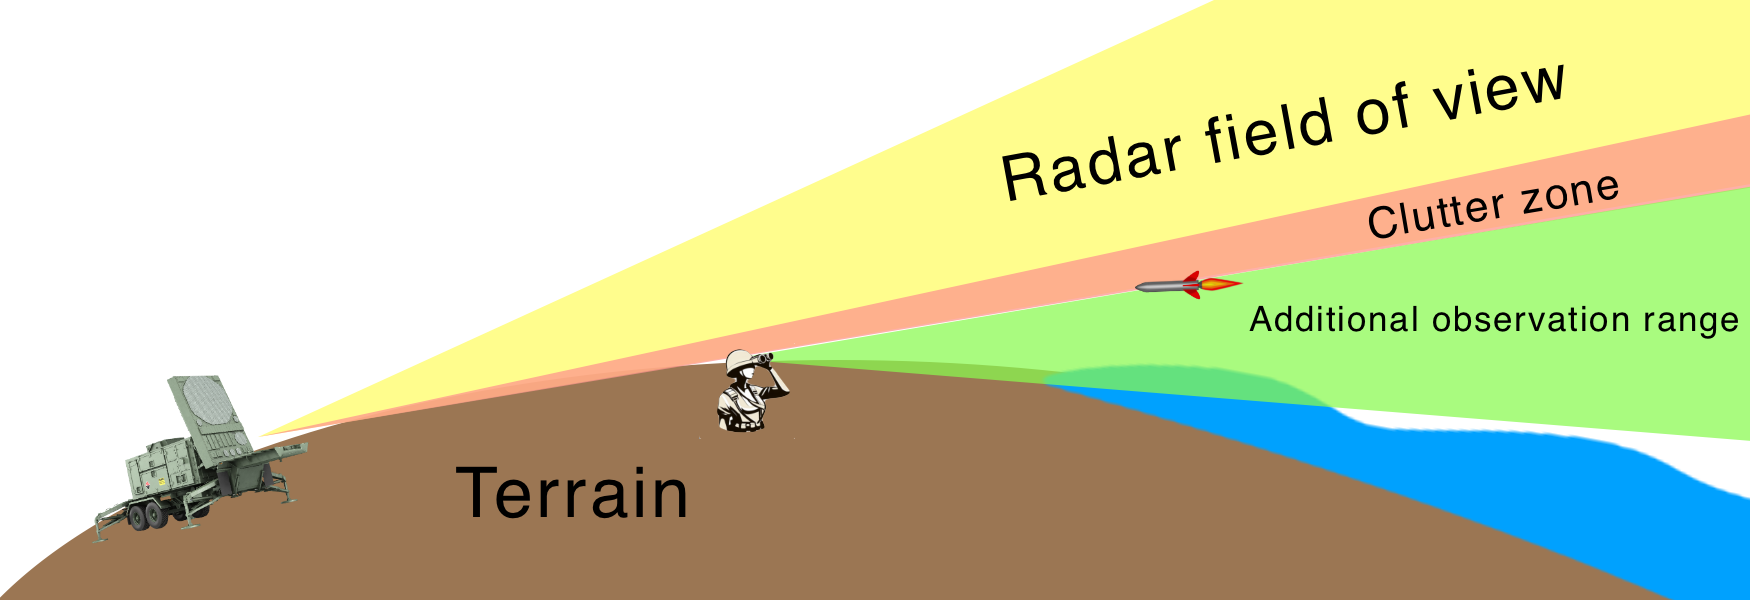
\includegraphics[width=0.9\linewidth]{pic/radar-presentation.png}
            \caption{Curvature of the Earth creates blind zones, necessitating additional sensors.}
        \end{figure}
        \pause
        \item \textbf{Problem:} Efficient integration of information from multiple sources.
    \end{itemize}
\end{frame}

\subsection*{Limitations}\begin{frame}[t]\frametitle{Technical Difficulties}
\framesubtitle{How Radars ``See'' the World}
    \begin{itemize}[<+->]
        \item<1-> Radars emit signals and read the target reflections.
        \item<2-> \alert{Noise} due to various factors (surface reflections, thermal emissions, random currents within components, etc.)
            \begin{center}
                \includegraphics<3>[width=0.5\linewidth]{pic/assignment-problem-red.png}
            \end{center}
    \end{itemize}
\end{frame}

\begin{frame}[t]\frametitle{Technical Difficulties}
\framesubtitle{Target-to-Measurement Assignment Problem}
    \begin{itemize}
        \item<1-4|only@1-4> But which measurements came from which target?
        \item<2|only@2> Is this the right assignment?
        \item<3|only@3> Or this way?
        \item<4|only@4> Maybe this?
        
        \item<5-6|only@5-6|alert@5>
            Harder still, radars can't inherently tell targets from noise.
    \end{itemize}
    
    \begin{center}
        \includegraphics<2|only@2>[width=0.5\linewidth]{pic/assignment-problem-red-1.png}
        \includegraphics<3|only@3>[width=0.5\linewidth]{pic/assignment-problem-red-2.png}
        \includegraphics<4|only@4>[width=0.5\linewidth]{pic/assignment-problem-red-3.png}
        \includegraphics<5-6|only@5-6>[width=0.4\linewidth]{pic/assignment-problem-gray.png}
    \end{center}

    \begin{itemize}
        \item<6|only@5-6>
            \textbf{Problem:} Having a framework that allows find the correct target-to-measurement assignment.
    \end{itemize}
\end{frame}
